%%%%%%%%%%%%%%%%%%%%%%%%%%%%%%%%%%%%%%%%%%%%%%%
%%% Template for lab reports used at STIMA
%%%%%%%%%%%%%%%%%%%%%%%%%%%%%%%%%%%%%%%%%%%%%%%

%%%%%%%%%%%%%%%%%%%%%%%%%%%%%% Sets the document class for the document
% Openany is added to remove the book style of starting every new chapter on an odd page (not needed for reports)
\documentclass[10pt,english, openany]{book}

%%%%%%%%%%%%%%%%%%%%%%%%%%%%%% Loading packages that alter the style
\usepackage[]{graphicx}
\usepackage[]{color}
\usepackage{listings}
\usepackage{float}
\usepackage{alltt}
\usepackage[T1]{fontenc}
\usepackage[utf8]{inputenc}
\setcounter{secnumdepth}{3}
\setcounter{tocdepth}{3}
\setlength{\parskip}{\smallskipamount}
\setlength{\parindent}{0pt}

% Set page margins
\usepackage[top=100pt,bottom=100pt,left=68pt,right=66pt]{geometry}

% Package used for placeholder text
\usepackage{lipsum}

% Prevents LaTeX from filling out a page to the bottom
\raggedbottom

% Adding both languages
\usepackage[english, italian]{babel}

% All page numbers positioned at the bottom of the page
\usepackage{fancyhdr}
\fancyhf{} % clear all header and footers
\fancyfoot[C]{\thepage}
\renewcommand{\headrulewidth}{0pt} % remove the header rule
\pagestyle{fancy}

% Changes the style of chapter headings
\usepackage{titlesec}
\titleformat{\chapter}
   {\normalfont\LARGE\bfseries}{\thechapter.}{1em}{}
% Change distance between chapter header and text
\titlespacing{\chapter}{0pt}{50pt}{2\baselineskip}

% Adds table captions above the table per default
\usepackage{float}
\floatstyle{plaintop}
\restylefloat{table}

% Adds space between caption and table
\usepackage[tableposition=top]{caption}

% Adds hyperlinks to references and ToC
\usepackage{hyperref}
\hypersetup{hidelinks,linkcolor = black} % Changes the link color to black and hides the hideous red border that usually is created

% If multiple images are to be added, a folder (path) with all the images can be added here 
\graphicspath{ {Figures/} }

% Separates the first part of the report/thesis in Roman numerals
\frontmatter


%%%%%%%%%%%%%%%%%%%%%%%%%%%%%% Starts the document
\begin{document}

%%% Selects the language to be used for the first couple of pages
\selectlanguage{english}

%%%%% Adds the title page
\begin{titlepage}
	\clearpage\thispagestyle{empty}
	\centering
	\vspace{1cm}

	% Titles
	% Information about the University
	{\normalsize Advanced Networking And Wireless Systems \\ 
		Computer Engineering Master Degree \\
		University of Pisa \par}
		\vspace{4cm}
	{\Huge \textbf{IoT Project}} \\
	%\vspace{1cm}
	%{\large \textbf{xxxxx} \par}
	\vspace{1cm}
	{\normalsize 6LoWPAN/RPL Wireless Sensor Network with CoAP Proxy for resource observing \par}
	\vspace{4cm}
    
    \centering 
\includegraphics[scale=0.4]{unipi_logo.png}
    
    \vspace{0.5cm}
		
	\pagebreak

\end{titlepage}

% Adds a table of contents
\tableofcontents{}

%%%%%%%%%%%%%%%%%%%%%%%%%%%%%%%%%%%%%%%%%%%%%%%%%%%%%%%%%%%%%%%%%%%%%%%%%%%%%%%%%%%%%%%%%%%%
%%%%%%%%%%%%%%%%%%%%%%%%%%%%%%%%%%%%%%%%%%%%%%%%%%%%%%%%%%%%%%%%%%%%%%%%%%%%%%%%%%%%%%%%%%%%
%%%%% Text body starts here!
\mainmatter

\chapter{Introduction}\label{chapt:sum}

The aim of this project is to design and implement a 6LoWPAN Wireless Sensor Network that uses RPL routing protocol with the Contiki development environment.
Every node is intended to sense the temperature value and to keep it as a CoAP resource. Moreover, with the CoAP protocol, a Proxy is implemented in order to "observe" the temperature values of the nodes and to forward when a Client request them.


\begin{figure}[h]
\centering
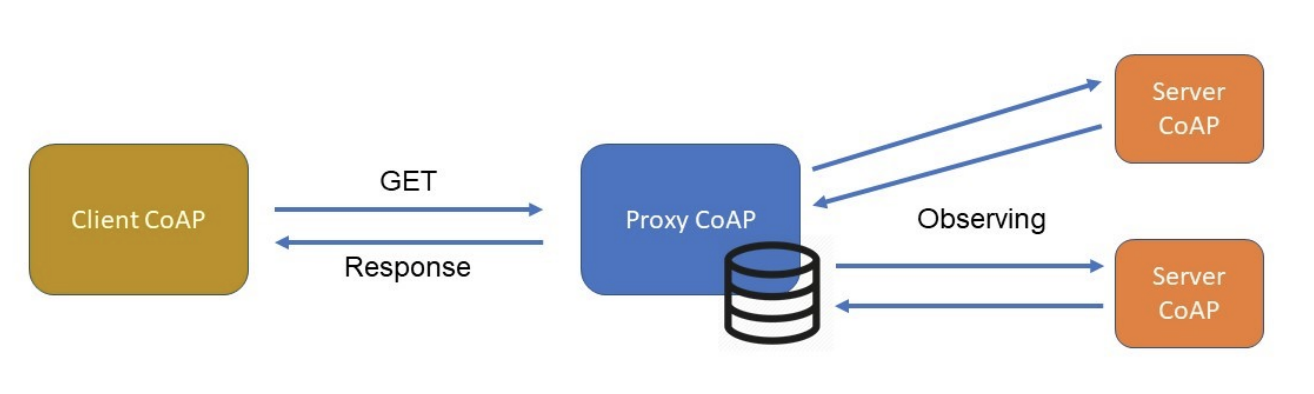
\includegraphics[scale=0.4]{application.png}
\caption{Sample of the application}
\end{figure}

Both the Proxy and the Client are implemented with Californium, the Java library for CoAP.
The Proxy, retrieves by observing the values of the temperature from every node deployed in the network and stores them in a private cache. When the Client request a temperature value of a certain node by specifying the ID of the node, to the Proxy by performing a GET operation, the latter one answer with the requested value.

\begin{figure}[h]
\centering
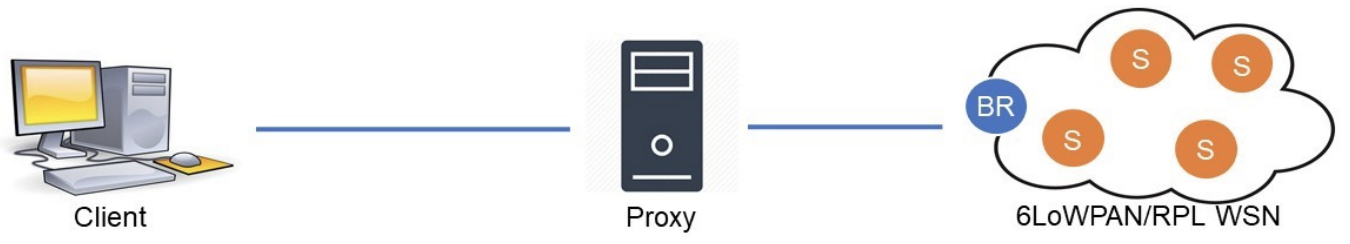
\includegraphics[scale=0.4]{architecture.png}
\caption{Architecture of the application}
\end{figure}

\chapter{Design}
\section{ClientCoAP}
The Client is implemented with JAVA. It allows to perform a request with a GET operation to the Proxy in order to obtain the temperature value of a node. The node of interest can be specified by inserting the numeric ID of it at runtime, the Client prepares the CoAP URI and forward the request to the Proxy.

\section{ProxyCoAP}
Also the Proxy is implemented with JAVA. At the startup it needs as an input the number of nodes deployed in the network in order to start the "observe" operation to every node. 
As already explained, the Proxy stores the last temperature value of every node in a cache. Hence, when a client makes a request for a value of a certain node, it will receive the last received value.
The cache is implemented as an array, every entry of the array correspond to a node in the WSN.

\section{CoAP Node}
A node is implemented with the Contiki environment (C language) using the Z1 mote as model. 
With the purpose of simulation, the temperature value is randomly generated and sent to the Proxy every time that a variation is detected.
The REST paradigm allows to keep the temperature value as a CoAP resource.

\chapter{Execution Tutorial}
In order to execute the project it is necessary to open the Cooja simulator on Contiki. Once the simulator is opened, we're now able to add the nodes and deploy the network. First of all the RPL border router is added to the network, then we can insert the other regular nodes. The nodes inserted in the WSN are around 20-30.

\begin{figure}[h]
\centering
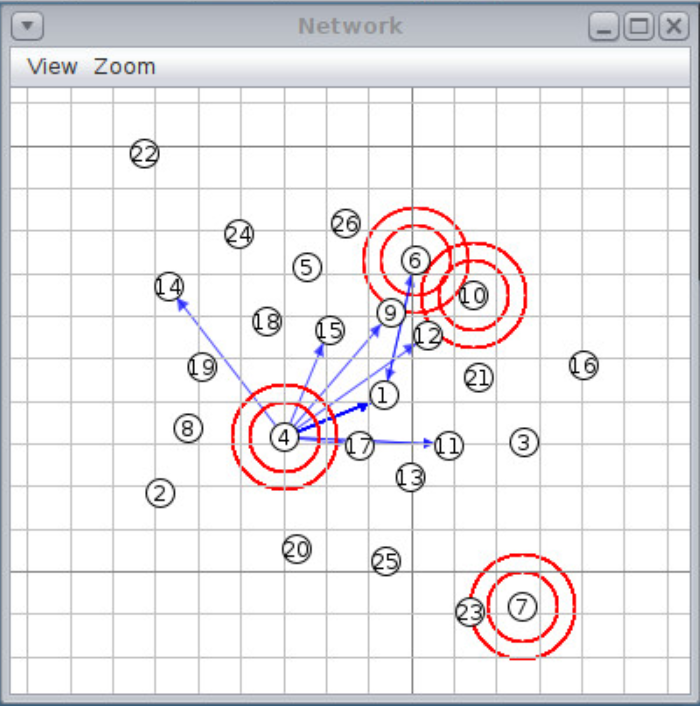
\includegraphics[scale=0.4]{network.png}
\caption{WSN deployed with Cooja simulator}
\end{figure}

It is necessary to define the Serial Socket port for the Border Router, by selecting \textit{Tools}, then \textit{Serial Socket (SERVER)} and finally select the Border Router and the listen port.
It is now neccessary to tun \textit{Tunslip6} by inserting the following command in a terminal:
\begin{lstlisting}
make connect-router-cooja PREFIX="abcd::1/64"
\end{lstlisting}
This is for creating the connection between the mote (border router) and the host.
It is reccomended now to start the simulation in Cooja and give some time before proceeding in order to create all the routes.

\begin{figure}[H]
\centering
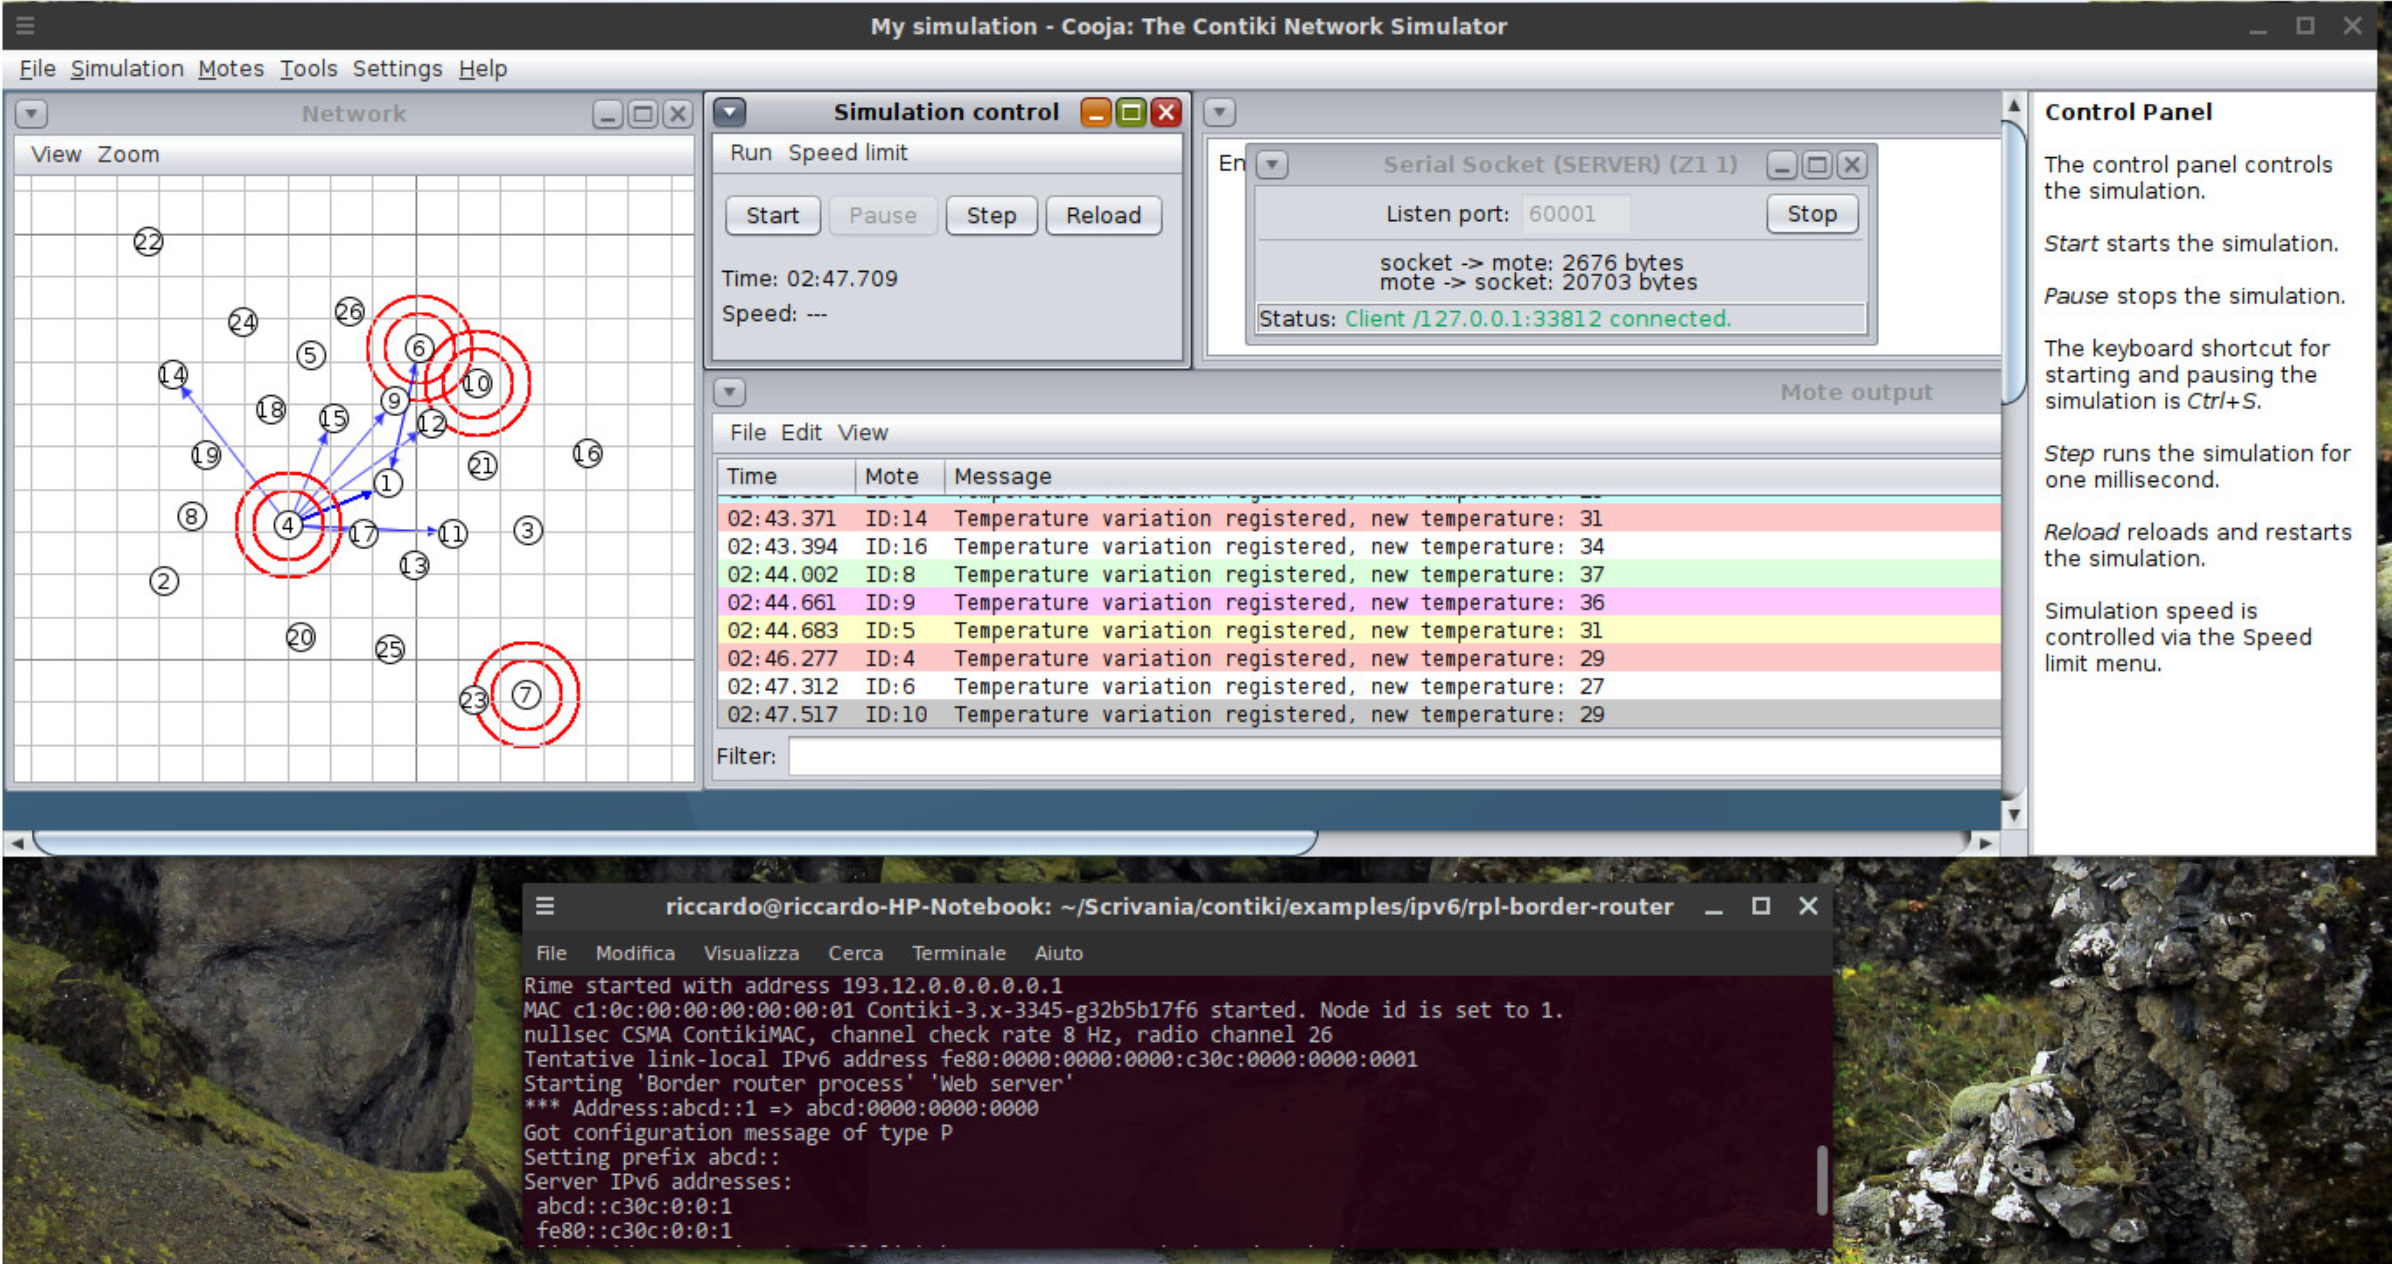
\includegraphics[scale=0.2]{simulation.png}
\caption{The running simulation in Cooja}
\end{figure}

Now it is possible to run the Proxy and the Client.
When the Proxy starts, it asks as an input the number of nodes deployed in the network. Once the number is inserted, it will start with the "observe" operation to the nodes and will report the temperature value of everyone.

\begin{figure}[H]
\centering
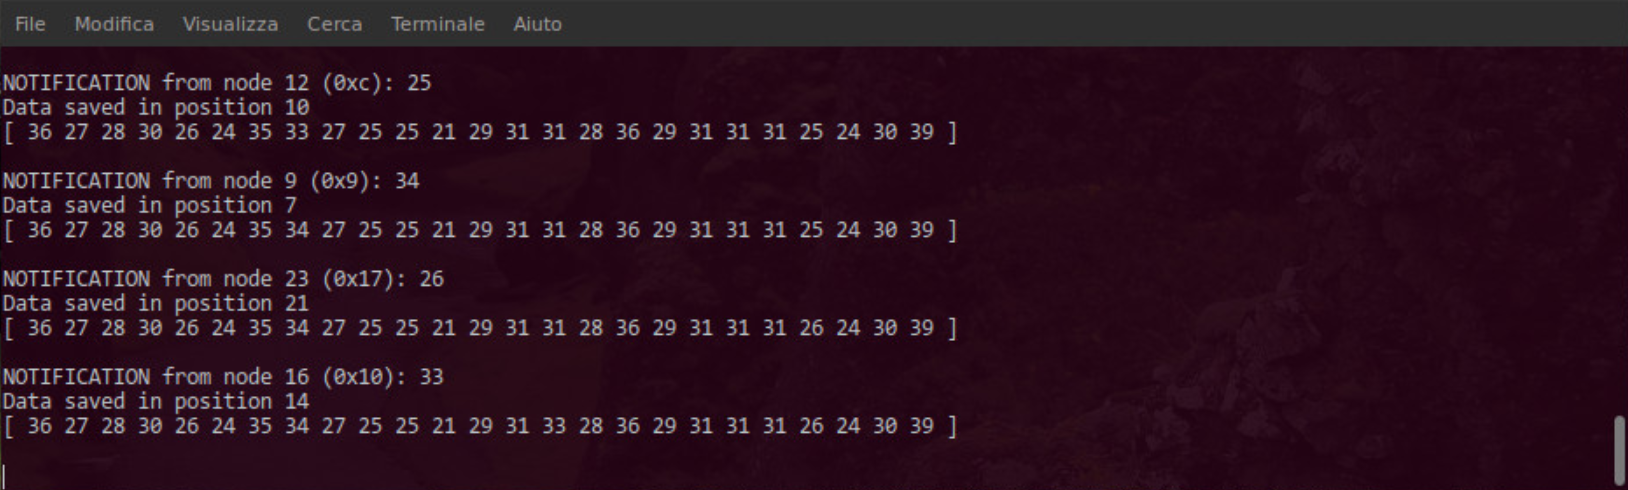
\includegraphics[scale=0.4]{proxy.png}
\caption{Sample of a Proxy execution with 25 nodes deployed}
\end{figure}

The client, at runtime, can request the temperature value of every node with a GET operation and the Proxy will reply by taking the last received value from the cache.

\begin{figure}[H]
\centering
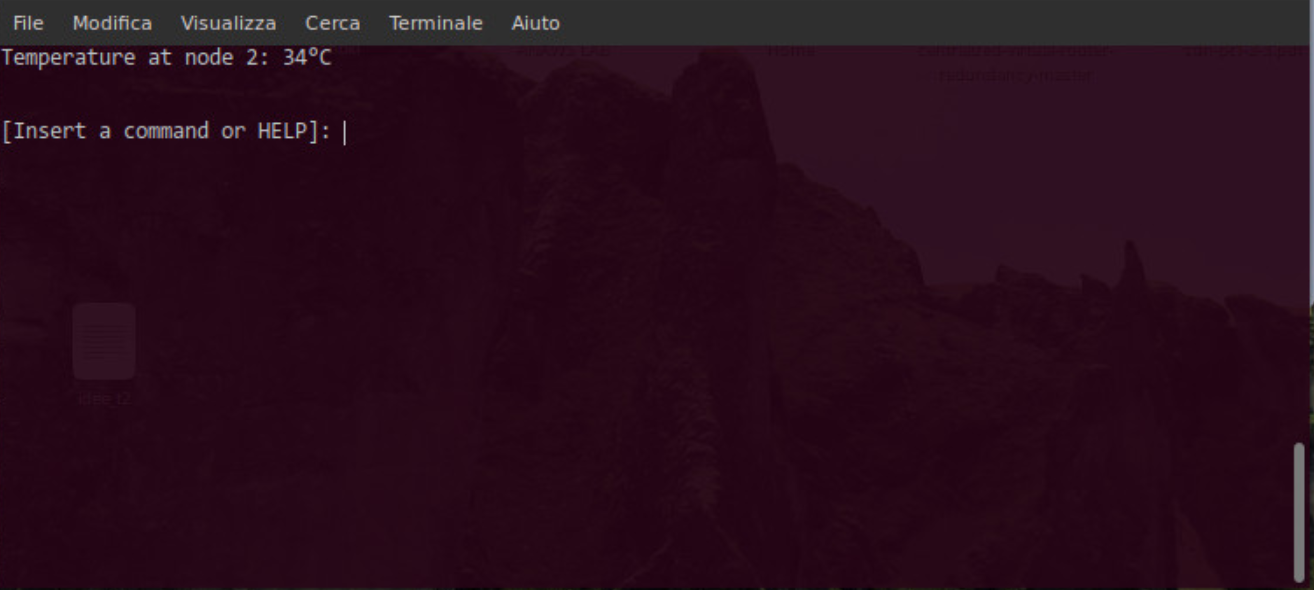
\includegraphics[scale=0.4]{client.png}
\caption{Sample of a Client request for a temperature value}
\end{figure}



\end{document}
